\documentclass[12pt]{article}

\pagestyle{empty}
\setcounter{secnumdepth}{2}

\topmargin=0cm
\oddsidemargin=0cm
\textheight=22.0cm
\textwidth=16cm
\parindent=0cm
\parskip=0.15cm
\topskip=0truecm
\raggedbottom
\abovedisplayskip=3mm
\belowdisplayskip=3mm
\abovedisplayshortskip=0mm
\belowdisplayshortskip=2mm
\normalbaselineskip=12pt
\normalbaselines

\usepackage{graphicx}
\usepackage{float}
\usepackage{titlesec}
\usepackage{lscape}

\setcounter{secnumdepth}{3}
\pagenumbering{arabic}
\pagestyle{plain}

\begin{document}

\vspace*{0.5in}
\centerline{\bf\Large Design Document}

\vspace*{0.5in}
\centerline{\bf\Large Team PB-PI}

\vspace*{0.5in}
\centerline{\bf\Large March 18, 2018}

\vspace*{1.5in}
\begin{table}[htbp]
\caption{Team}
\begin{center}
\begin{tabular}{|r | c|}
\hline
Name & ID Number \\
\hline\hline
Alissa Bellerose & 27377320 \\
Sabrina D'Mello & 27739486 \\
Melanie Damilig & 40032420 \\
Tobi Decary-Larocque & 27407645 \\
Zain Farookhi & 26390684 \\
Giulia Gaudio & 27191766 \\
Jason Kalec & 40009464 \\
Damian Kazior & 40016168 \\
Johnny Mak & 40002140 \\
Philip Michael & 40004861 \\
Ramez Nicolas Nahas & 26718108 \\
Steven Tucci & 40006014 \\
Shunyu Wang & 40043915 \\
\hline
\end{tabular}
\end{center}
\end{table}

\clearpage
\tableofcontents
\clearpage

\section{Introduction}
The primary goal of this project is to create an application which allows students to keep track of their money. The MyMoney application allows students to create an account which provides them with different options to keep track of their money and spending habits through the graphical user interface. The application allows the user to create a transaction, either deposit or withdraw. It will also allow the user an option to display balance, show or export transaction history and clear history. 

\subsection{Purpose}
The purpose of this document is to provide details on the architectural design, software design and internal design of the MyMoney application. The software architecture that was chosen for the application will be described in high level detail and a class diagram will be depicted. The software interface will have screenshots of the graphical user interface and a high level description of how the user will interacts with the system.


\subsection{Scope}
This document is intended to provide a basis for implementation. The architecture and software processes will be explained in great detail in order to facilitate implementation and be an effective reference tool. 


\subsection{Definitions and Abbreviations}

\subsubsection{Definitions}
\begin{table}[H]
\caption{Definitions}
\begin{center}
\begin{tabular}{|p{3cm}|p{12cm}|}
\hline
Term & Definition \\
\hline\hline
Model View Controller & The architecture used in the MyMoney application. It consists of 3 individual components the model, the view and the controller.  \\
\hline

\end{tabular}
\end{center}
\end{table}

\subsubsection{Abbreviations}

\begin{table}[H]
\caption{Abbreviations}
\begin{center}
\begin{tabular}{|p{3cm}|p{12cm}|}
\hline
Abbreviation & Term \\
\hline\hline
GUI & Graphical User Interface  \\
\hline
MVC & Model View Controller \\
\hline
UML & Unified Modeling Language \\
\hline
ORM & Object Relational Mapping \\
\hline
API & Application Programming Interface \\
\hline
CRUD & Create, Read, Update, Delete \\
\hline
SQL & Structured Query Language \\
\hline

\end{tabular}
\end{center}
\end{table}


\subsection{References}

Pressman, Roger S. Software Engineering: A Practitioner's Approach. 5th ed. Toronto: McGraw-Hill, 2001. 

Larman, Craig. Applying UML and patterns: an introduction to object-Oriented analysis and design and the unified process. Prentice-Hall, 2005.


\subsection{Overview}
This document is divided into three major parts; the architectural design, the detailed design and the dynamic design scenarios. The architectural and software design will be described in detail in their respective individual parts.


\section{Architectural Design}

\subsection{Architectural Diagram}
The MyMoneyApp uses a variant of the MVC architecture with an observer pattern to notify of data changes. The MVC pattern is known as the Model-View-Controller pattern.  Along with the MVC architecture the application also has singleton patterns. The singleton design pattern is used for only instantiating one object from a class. The singleton pattern was used for the creating the default GUI layout for the user and the initial connection to the applications database. 

\begin{figure}[h!]
  \centering
  \includegraphics[width=110mm]{MVC_new.png}
  \caption{MVC Diagrams}
\end{figure}

\begin{landscape}
%% We'll need a way to put the class diagram as the whole page
\begin{figure}[h!]
  \centering
  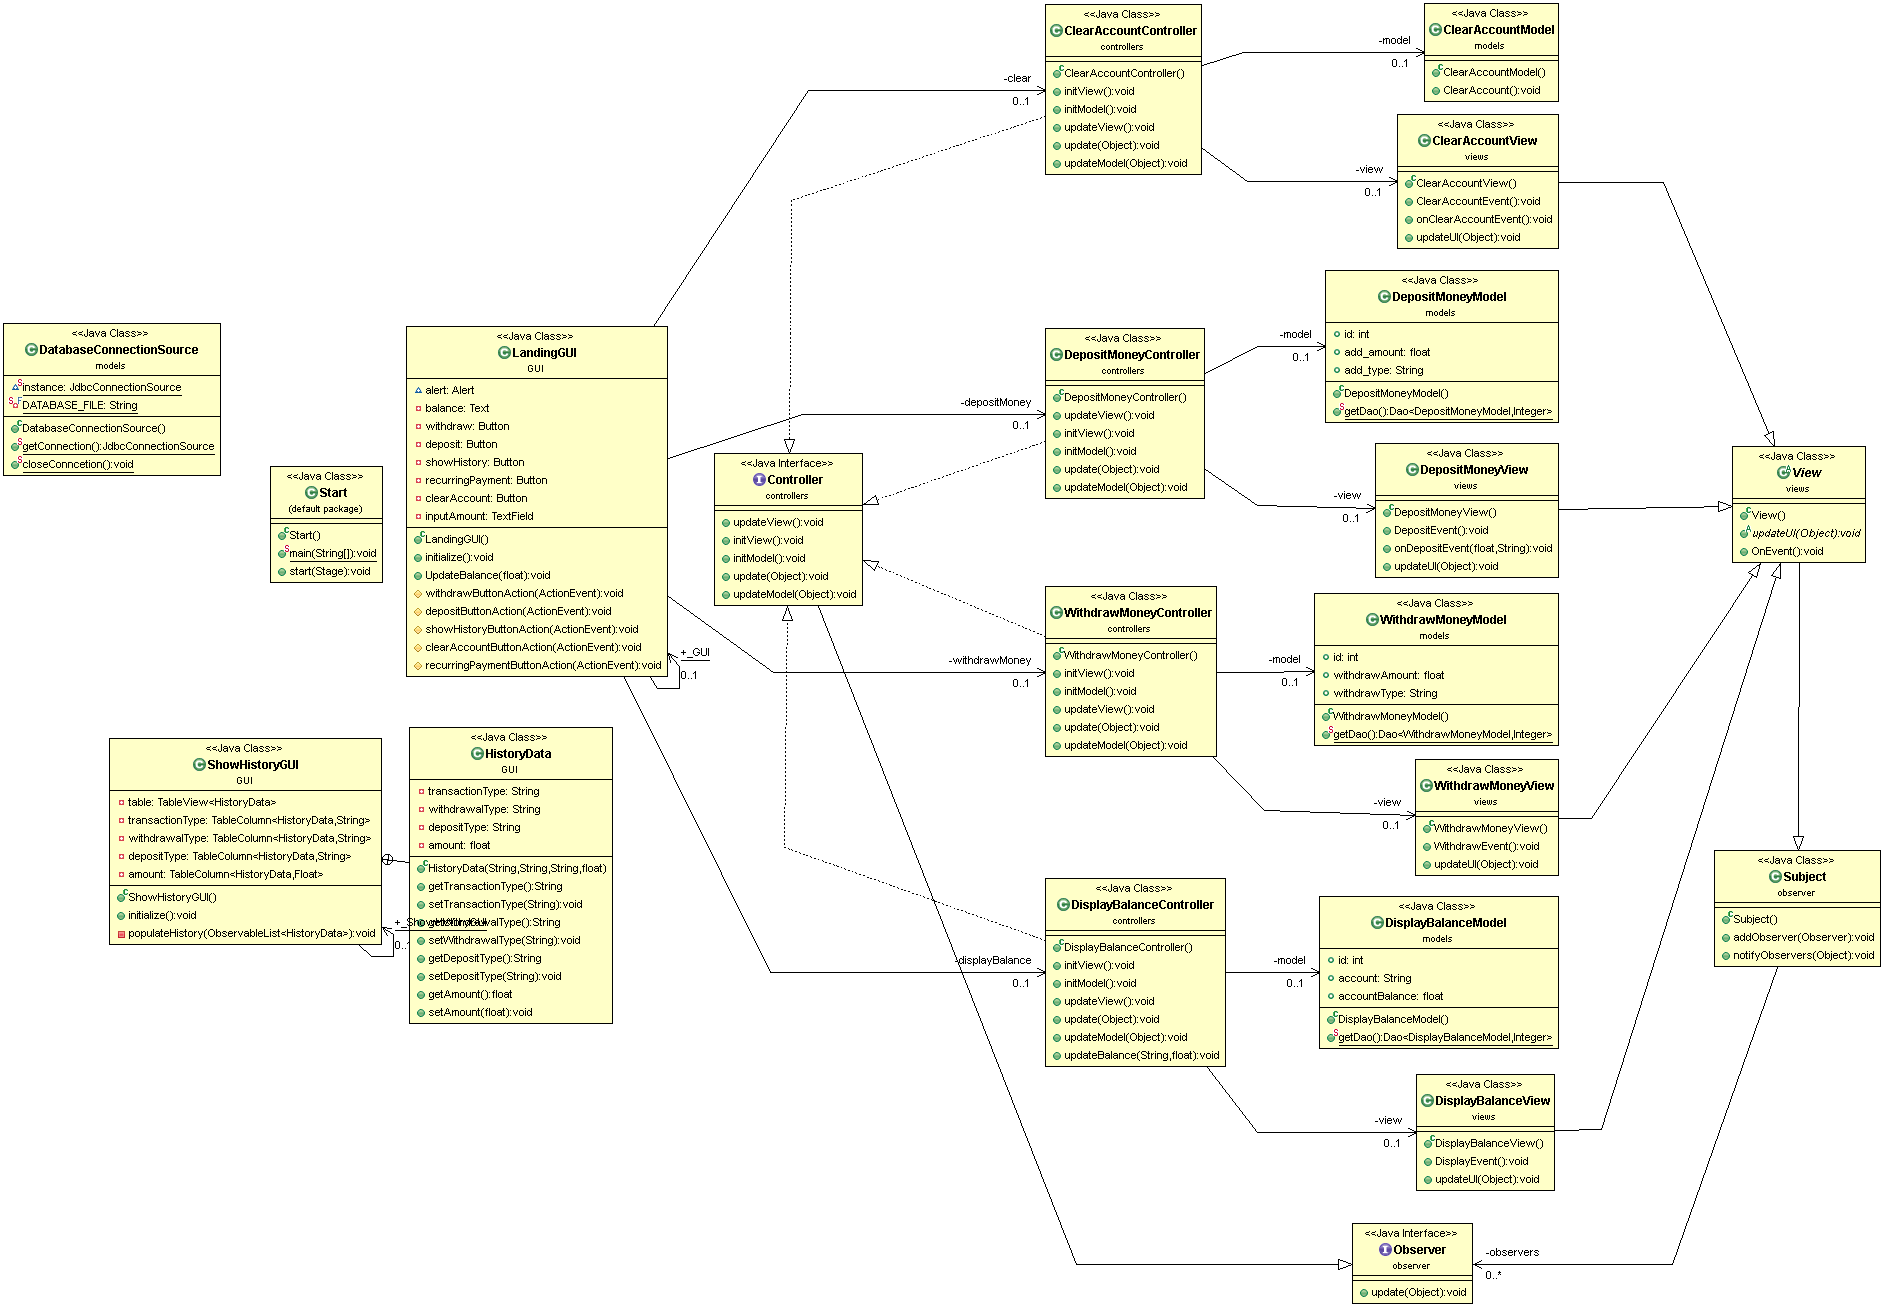
\includegraphics[width=250mm]{class_diagram.png}
  \caption{Class diagram}
\end{figure}
\end{landscape}



\subsubsection{Model}
The model component is where we store our business models and data. For that, we use an abstraction known as ORM (Object Relational Mapping). The ORM allows us to perform CRUD operations on our data without writing hardcoded specific database queries. This allows us to perform queries on a higher abstraction level and be able to switch our data store without having to rewrite new query code. 


\subsubsection{View}
The view component layer is where the user interacts with the system. In our case this is the GUI, but the view layer does not necessarily have to be a GUI. The view displays our models, collection of models, or any mix of model data. Since the user interacts with the view, all view logic at the view layer. As a result, when a user presses a button, the view captures the event, then it creates a message and passes it to the controller to handle the event.  


\subsubsection{Controller}
The controller component acts as an intermediary between the view and model. When an event occurs in the view, the view passes the message to the controller. The controller reads the message, and reflects the changes from the view across the model. The controller then updates the model data where it gets automatically updated into our database. Once the model gets updated, the controller takes any changes from the model and sends a message back to the view with the new updated model data. The view then takes this message and reflects the view/gui changes with the data.


\subsubsection{View/Controller Interface}

In the classic version of MVC, the model is the subject, and the view is the observer that subscribes to the model. Our version does not do this and will be further explained in the rationale.

\subsubsection{Controller/Model Interface}

The controller does not directly manipulate the model through database queries, but instead it manipulates the model’s high level ORM API.

\subsection{Rationale}
MyMoneyApp uses an evolved version of the MVC architecture with the observer pattern. It allows us to independently manage business logic from the view logic. We could create new views without ever worrying about how the controller and model work. This allows for new controllers and models to be created, tested, debugged, and integrated in parallel.
Though our architecture may not be the same MVC as stated in Larman’s book, it uses a newer modern version variant of MVC, in which the controller acts as a mediator between the model and view. The view causes an event, delegates to the controller, the controller modifies the model, then the controller notifies the view of the model changes. The diagrams are a good visual representation of this new structure. We can see that we don't have a connection between our model and view. That is because the controller handles it. In the original MVC pattern, the model directly notifies the view through the observer pattern. For our structure, our controller notifies the view through the observer pattern. This removes the coupling between our model and view and allows the controllers and models to be tested much easier. Given that the model isn’t in charge of notifying the view, one would think that the views would become out of date. However it does not, because it is now the controller notifying its dependant views.


\subsection{Subsystem Interface Specifications}
All the subsystems interact with a message passing interface. Each view has a custom data type message that is passes to the other subsystems. The corresponding controller should expect the custom message and handle it appropriately. When messages are passed around, they are passed as high level Object class types, the views and controllers must down cast the object to its expected message type/class.


\subsubsection{View Interface Subsystem}

\begin{table}[H]
  \caption{updateUi method spec}
  \begin{center}
    \begin{tabular}{|l|p{10cm}|}

      \hline
      \bf Method: & void updateUI(Object data)\\
		\hline
      \bf Purpose: & To notify the view that it should update its view state with the current data message.
This is the controller to view interface. This is used when the controller sends a message to the view.\\
\hline
      \bf Parameters: & Object data. The data/message that the current view should unpack/cast and update its state with.The view should cast the object to its own object type.\\
		\hline
      \bf Valid data: &  An object of type that is known to the view and controller\\
      \hline
      \bf Invalid data: &  Null, or an unknown data message type. The view should handle invalid data in an expected manner, and should not throw any exceptions up the system interface.\\
      \hline

    \end{tabular}
  \end{center}
\end{table}

\begin{table}[H]
  \caption{notifyObservers method spec}
  \begin{center}
    \begin{tabular}{|l|p{10cm}|}
      \hline
      \bf Method: & void notifyObservers(Object data)\\
		\hline
      \bf Purpose: &  Notify all dependent observers/controllers with a new message/data. This is the view to controller interface. This is used when the view wants to send a message to the controller.\\
		\hline
      \bf Parameters: & Object data. The data/message that the current view sends to its controller when the view wants to notify the controller of a view event or change.\\
		\hline
      \bf Valid data: &  An object of type that is known to the view and controller\\
      \hline
      \bf Invalid data: & Null, or an unknown data message type. The view should handle invalid data in an expected manner, and should not throw any exceptions up the system interface.\\
      \hline

    \end{tabular}
  \end{center}
\end{table}

\begin{table}[H]
  \caption{addObserver method spec}
  \begin{center}
    \begin{tabular}{|l|p{10cm}|}
      \hline
      \bf Method: & void addObserver(Observer observer)\\
		\hline
      \bf Purpose: & Add an observer/controller to the current subject/view.\\
		\hline
      \bf Parameters: & Observer observer. The controller that subscribes to the view/subject’s events or changes.\\
		\hline
      \bf Valid data: & An observer object that should be expected to handle the view’s messages.\\
      \hline
      \bf Invalid data: &Null, or an unknown controller type that would not know how to handle the view’s messages.\\
      \hline

    \end{tabular}
  \end{center}
\end{table}

\subsubsection{Controller Interface Subsystem}

\begin{table}[H]
  \caption{initModel method spec}
  \begin{center}
    \begin{tabular}{|l|p{10cm}|}
      \hline
      \bf Method: & void initModel()\\
		\hline
      \bf Purpose: & Initialize any model or models that the controller needs to update or create.\\
		\hline
      \bf Parameters: & None.\\
		\hline
    \end{tabular}
  \end{center}
\end{table}

\begin{table}[H]
  \caption{initView method spec}
  \begin{center}
    \begin{tabular}{|l|p{10cm}|}
      \hline
      \bf Method: & void initView()\\
		\hline
      \bf Purpose: &  Initialize the view and setup any needed view logic.\\
		\hline
      \bf Parameters: & None.\\
		\hline
    \end{tabular}
  \end{center}
\end{table}

\begin{table}[H]
  \caption{updateView method spec}
  \begin{center}
    \begin{tabular}{|l|p{10cm}|}
      \hline
      \bf Method: & void updateView()\\
		\hline
      \bf Purpose: & Tells the controller's attached view to update its ui. This method is called after any model changes have happened, and the view needs to reflect these changes.\\
		\hline
      \bf Parameters: & None.\\
		\hline
    \end{tabular}
  \end{center}
\end{table}

\begin{table}[H]
  \caption{update method spec}
  \begin{center}
    \begin{tabular}{|l|p{10cm}|}
      \hline
      \bf Method: & void update(Object data)\\
		\hline
      \bf Purpose: & Update the controller/observer data/state. Update the model with the new changes from the view’s data/message.\\
		\hline
      \bf Parameters: & Object - data, this is the corresponding data message passed from the view's notifyObserver(Object data) call the object is usually going to be type casted to the specified data type depending on the what the view's data is. the data reflects the state of the view\\
		\hline
      \bf Valid data: & An object of type that is known to the view and controller\\
      \hline
      \bf Invalid data: &  Null, or an unknown data message type. The controller should handle invalid data in an expected manner, and should not throw any exceptions up the system interface.\\
      \hline

    \end{tabular}
  \end{center}
\end{table}


\subsubsection{Model Interface Subsystem}
For our model, we are using an ORM called ORMLite. It allows us persist our business objects to a database using a high level api and avoid us having to write our own custom and insecure SQL queries. 

\subsection{System Topology}
The MyMoneyApp is to be used by a single user and ran on a single computer. There will be no need for networked communications or internet connections for the app to work. This allows us to easy distribute the app and integrate all the components into a single executable.


\section{Detailed Design}
The primary User Interface used in the system design, was created using Java FX, which is quite similar to Java Swing. This GUI gives users the ability to interact with the core necessary aspects of the system in order to obtain a satisfactory user experience.

User interactions:\\ \\
The user may press “Withdraw Amount” to reveal the withdrawal interface where the user may then enter an amount, a type of withdrawal and an optional transaction description, then click “Done” to confirm the withdraw. A user may alternatively press “Cancel” to discard the withdraw.\\ \\
The user may press “Deposit Amount” to reveal the withdrawal interface where the user may then enter an amount, a type of withdrawal and an optional transaction description, then click “Done” to confirm the withdraw. A user may alternatively press “Cancel” to discard the withdraw.\\ \\
The user may press “Show History” to bring up a list of past transactions as well as all relevant information regarding each transaction. The user can sort by each category such as date or type.\\ \\
The user may press “Clear Account” to bring the app back to original settings, clear history and set the balance back to 0.\\ \\
The user has the option to press “Export History” to write the past transactions to a CSV file which can then be viewed as a text file or it may be opened in excel\\




\subsection{Main Interface}
The systems main interface is composed of various elements required to manage ones money.
There are basic options such as “Withdraw Amount”, “Deposit Amount” and “Show Balance”. There are also advanced options such as “Clear Account” and “Export History”. The User interface has a “Amount” box where one can enter the amount of money they may wish to deposit or withdraw as well as a type of deposit or withdraw “Bill Payment” being an example as well as an optional “Transaction Description”. The app is constantly displaying the users “Current Balance” so they will constantly be aware of how much money they currently have in green if it is positive or in red if the user is in debt.


% Screenshot of the app window
\begin{figure}[h!]
  \centering
  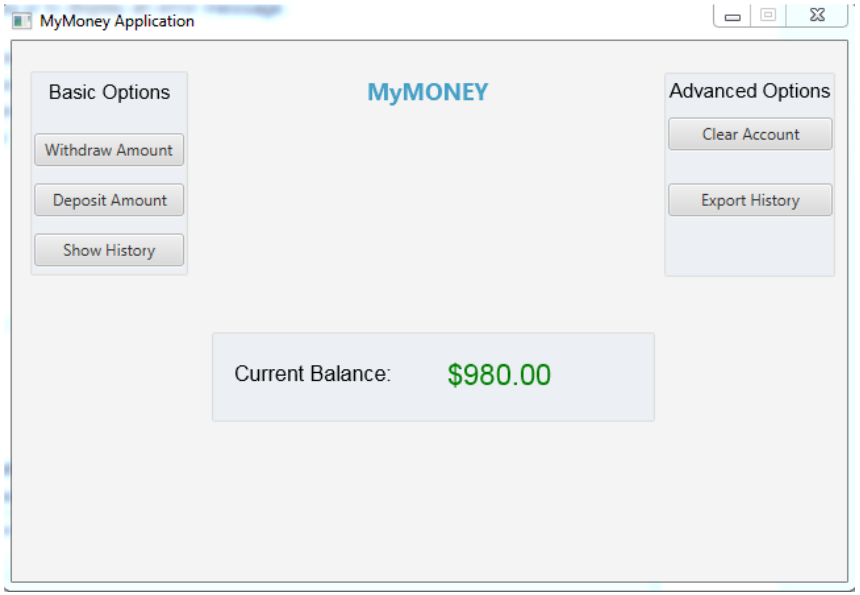
\includegraphics[width=110mm]{maininterface.PNG}
  \caption{MyMoney Application Window}
\end{figure}


\subsubsection{Basic Options}
The basic options subsection of the GUI is displayed as such all functionality that the user will be using frequently such as deposit, withdraw and show history will be available here.

% Basic Options Image
\begin{figure}[h!]
  \centering
  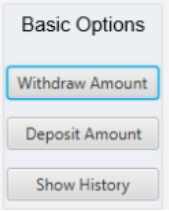
\includegraphics[width=40mm]{basicoption.PNG}
  \caption{Basic Options}
\end{figure}

\subsubsection{Advanced Options}
The advanced options subsection of the GUI is displayed as such all functionality that is not frequented often such as “Export History” and “Clear Account” will be available here.

% Advanced Options Image
\begin{figure}[h!]
  \centering
  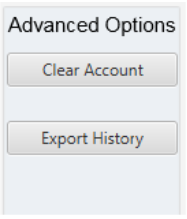
\includegraphics[width=40mm]{advanceoption.PNG}
  \caption{Advanced Options}
\end{figure}

\subsubsection{Withdraw Button}
The withdraw button of the basic options subsection when clicked on will display to the user the withdraw interface.

% Withdraw button Image
\begin{figure}[h!]
  \centering
  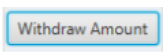
\includegraphics[width=40mm]{withdrawbutton.PNG}
  \caption{Withdraw Button}
\end{figure}

The Withdrawal interface is where the user will chose the properties and information for their transaction. The user must specify an amount to withdraw and the type of withdraw for example a “Bill Payment” and the user may enter an optional transaction description to better describe their withdrawal. Once finished, the user may click ok to confirm the withdraw or press cancel to go back to the main interface and discard the withdraw.

% Withdraw Interface Image
\begin{figure}[h!]
  \centering
  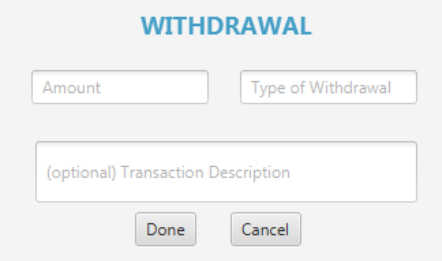
\includegraphics[width=60mm]{withdrawinterface.PNG}
  \caption{Withdraw Interface}
\end{figure}

\subsubsection{Deposit Button}

The deposit button of the basic options subsection when clicked on will display to the user the deposit interface.

% Deposit button Image
\begin{figure}[h!]
  \centering
  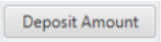
\includegraphics[width=40mm]{depositbutton.PNG}
  \caption{Deposit Button}
\end{figure}

The Deposit interface is where the user can specify amount, type of withdrawal and transaction description for their transaction. The user must specify an amount to deposit and the type of deposit for example a “Paycheck” and the the user may enter an optional transaction description to better describe their deposit once finished the user may click ok to confirm the deposit or press cancel to go back to the main interface and discard the deposit.

% Deposit Interface Image
\begin{figure}[h!]
  \centering
  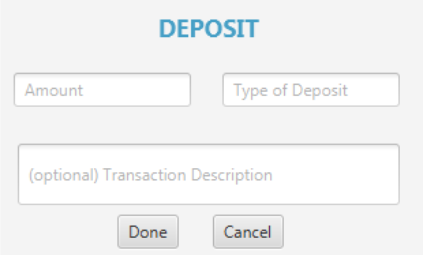
\includegraphics[width=65mm]{depositinterface.PNG}
  \caption{Deposit Interface}
\end{figure}

\subsubsection{Show History Button}
The show history button of the basic options subsection when clicked upon will show the past transactions that the user has done such as withdrawals and deposits.

% Show history button Image
\begin{figure}[h!]
  \centering
  
\includegraphics[width=40mm]{showhistorybutton.PNG}
  \caption{Show History Button}
\end{figure}

The history interface will be displayed upon clicking “Show History”. The history interface will display all past transactions as well as all relevant information regarding each past transaction. Each transaction will be displayed ordered by date, there is the option to order by type, description, etc. Each transaction will have information regarding the date that it was made, whether it was a withdraw or a deposit, the description of the transaction, the amount, and the type of withdraw or type of deposit.

% Show history button Image
\begin{figure}[h!]
  \centering
  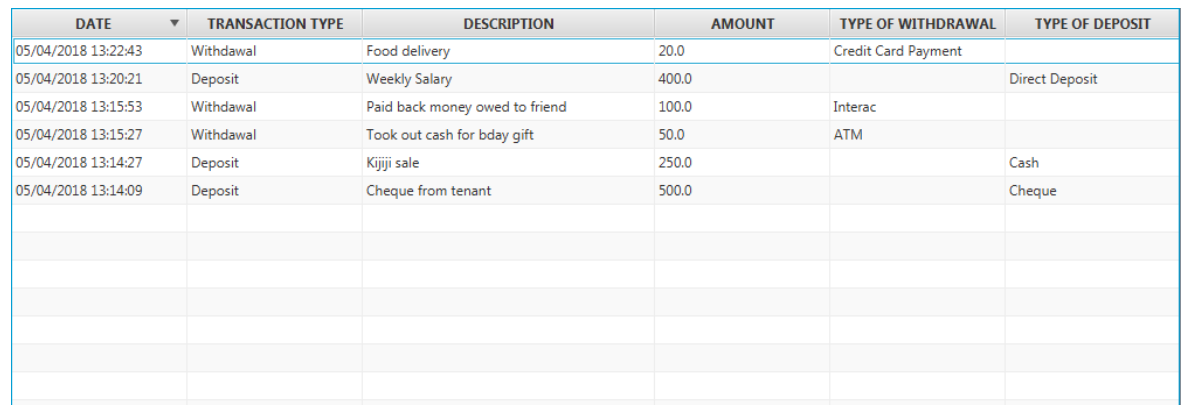
\includegraphics[width=180mm]{showhistoryinterface.PNG}
  \caption{Show History Interface}
\end{figure}

\subsubsection{Export History}
The “Export History” button when clicked on will take all past transactions and write them to a csv file which can then be imported into excel.

% Export Button Image
\begin{figure}[h!]
  \centering
  
\includegraphics[width=40mm]{exportbutton.PNG}
  \caption{Export Button}
\end{figure}

\subsubsection{Clear Account}
The clear account button of the advanced options subsection will delete the current account and reset the application back to the clear default state.

% Export Button Image
\begin{figure}[h!]
  \centering
  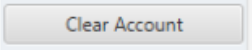
\includegraphics[width=40mm]{clearaccount.PNG}
  \caption{Export Button}
\end{figure}


\subsubsection{Enter Amount Field}
The amount field located in the center of the GUI in the deposit and withdraw interface is where the amount is typed to perform operations on the current balance such as typing in a certain amount to manipulate the current balance and perform the transaction.

% Enter Amount Image
\begin{figure}[h!]
  \centering
  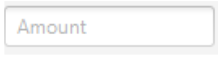
\includegraphics[width=40mm]{amount.PNG}
  \caption{Enter Amount Field}
\end{figure}

\subsubsection{Type of Deposit/Withdraw}
The “Type of Deposit” and “Type of Withdraw” is where the user would specify what type of withdraw or deposit they intend to apply, for example “Pay Check” or “Bill Payment” which will then be inserted into the database to quickly describe the deposit or withdraw.

% Type of Deposit/Withdraw Image
\begin{figure}[h!]
  \centering
  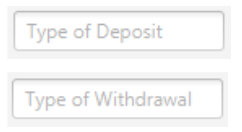
\includegraphics[width=40mm]{typewd.PNG}
  \caption{Type of Deposit/Withdraw Field}
\end{figure}

\subsubsection{Transaction Description}
The optional “Transaction Description” text box is used to describe a transaction if the type of deposit or withdrawal is not enough. This will be inserted into the database to thoroughly describe the transaction being inserted.

% Transaction Description Image
\begin{figure}[h!]
  \centering
  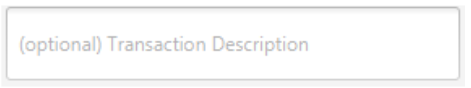
\includegraphics[width=70mm]{transdescrib.PNG}
  \caption{Transaction Description}
\end{figure}


\subsubsection{Current Balance Field}
The current balance field at the bottom of the GUI is where the user’s current balance is displayed. The field will display green if the current balance is greater than 0 and red if the current balance is less than 0.

% Current Balance Field Image
\begin{figure}[h!]
  \centering
  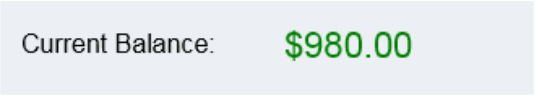
\includegraphics[width=90mm]{currentbalance.PNG}
  \caption{Current Balance Field}
\end{figure}


\section{Dynamic Design Scenarios}
As explained, our software offers many functionalities that allows the user to interact with it. These functionalities were developed based on the gathered user stories. It includes: Deposit Amount, Withdraw Amount, Show Balance, Show History, Clear History, and Display GUI. 

\subsection{Deposit Amount}

Our software provides the user with basic functionality such as “Deposit Amount” which simply allows the user to input an amount along with certain details to be saved as a deposit as explained above in the Main Interface section. Once stored, the data can be used by other functionalities to extend the user intractability with the system. 


\subsubsection{Deposit Amount - Sequence Diagram}

\begin{figure}[h!]
  \centering
  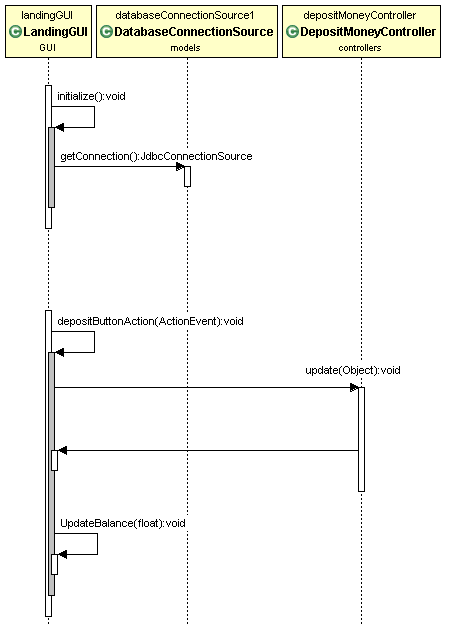
\includegraphics[width=90mm]{deposit_sequence.png}
  \caption{Deposit Sequence Diagram}
\end{figure}
\clearpage

The Deposit Amount use case is a basic functionality that is invoked from the GUI. When the GUI is launched, it establishes a connection with the database and then waits for user inputs. Once the user entered an amount into the Deposit’s input box and confirmed their action by pressing the “Deposit Amount” button, the function depositButtonAction(ActionEvent) is called which tells the DepositMoneyController to update the Model. When updated, the DepositMoneyController will signal the GUI that the information has been successfully updated and that it needs to display the new information. The GUI will then call UpdateBalance(float) which will finally update the displayed balance to reflect the new amount.



\subsection{Withdraw Amount}
Similar to the “Deposit Amount” use case, “Withdraw Amount” is another basic functionality that allows the user to interact with the system. It requires the user to input a withdrawal amount which is saved into the “Withdraw” section of the account. 

\subsubsection{Withdraw Amount - Sequence Diagram}
\begin{figure}[h!]
  \centering
  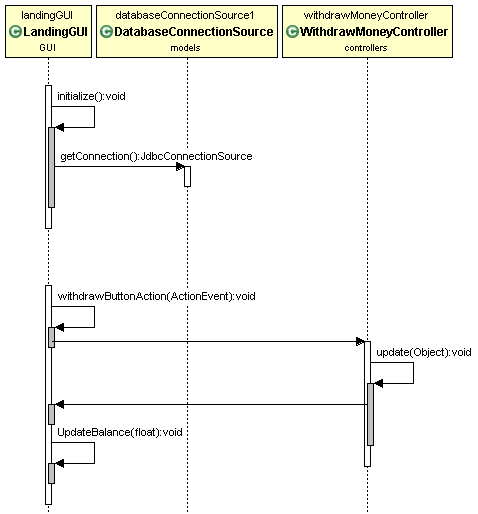
\includegraphics[width=100mm]{withdraw_sequence.png}
  \caption{Withdraw Sequence Diagram}
\end{figure}
\clearpage

This use case functions very similarly to the “Deposit Amount” use case. It establishes a database connection when the GUI is launched and waits for user inputs. Once a withdrawal amount has been entered and confirmed by the user, it triggers the withdrawButton(ActionEvent) function which informs the WithdrwaMoneyController to update the Model. The controller will then update the model and inform the GUI that the changes has been successfully applied. The GUI will then call UpdateBalance(float) function which will update the displayed balance to reflect the new amount.

\subsection{Show Balance} 
“Show Balance” is a feature that allows the user to see the difference between their monthly earning and spending. This amount can be negative or positive to reflect the user’s monthly money situation. This use case solidifies the intent of our software which allows the user to know about their spending habits for a given period of time.

Additionally, the balance amount is shown on the main window of the software and is constantly updated when specific actions are made. For instance, a successful Deposit or Withdraw amount input would update the balance once the action is complete. 


\subsection{Show History} 
“Show History” is a functionality that allows the user to see all previous Deposit and Withdraw inputs to review certain purchases they have made or certain deposits they have forgotten for instance. When the “Show History” button is pressed, a new window containing the information will pop up on top of the main window. This new window is independent to the main window and can be freely manipulated by the user. 

Within this new window, it will display a table with all Deposit and Withdraw inputs since the beginning. The data is sorted by the input date from newest to oldest. The user can resume their normal activity with the software regardless of whether the “Show History” window is active or not. Although, if the user inputs more data with the history window still open, it will not display the new additions and would require the user to reopen the same window to see the changes.

\subsection{Sort History} 
After opening up the “Show History” window, the user has the choice to sort any column of the window. By default, the data is sorted by newest date but the user can opt to sort the data by either: date, transaction type, description, amount, type of withdrawal, or type of deposit. This functionality does not affect how the data is stored. It will only manipulate how the data is displayed to the user.  

\subsection{Export History} 
“Export History” is a functionality very similar to “Show History”. Just like the other functionality, it shows to the user all previous Deposit and Withdraw inputs but instead, exports this data into a CSV file. This file containing all the information can then opened into Microsoft Excel where the user can further analyze or archive his data. 

\subsection{Clear History}
“Clear History” is another functionality that allows the user to remove all data that has ever been saved into the software. This allows any old or unnecessary information to be removed allowing the user to only see recent information. By pressing the “Clear History” button, it will empty all tables within the database such as Deposit and Withdraw amounts. It is recommended that the user first exports their data before clearing their history. 

\subsection{Display GUI}
“Display GUI” is a feature that allows the user to easily interact with the system.The GUI simplifies the number of steps required for the user to carry out an action on the software by allowing them to simply type into input boxes and press on buttons to confirm their actions.This feature also compacts all other features and functionalities into one window which greatly improves the user’s experience. 

\section{Conclusion}
The MyMoneyApp was created for users to be able to manage their personal financials. The App allows them to constantly keep track of their money that has been deposited and withdrawn. The user can also view their history of their transactions as well as view their balance. Another feature of this application is that it allows the user to clear their history of transactions. This document was to analyse the design of the application.

The primary user interface of the MyMoneyApp was created with Java FX. The GUI allows easy and quick access for the user to deposit, withdraw, view balance, view history and clear transactions. 
 
The MyMoneyApp design documentation was created to express the major design implementation that was used in creating this money management application for an average everyday user.


\end{document}